\documentclass[aspectratio=169]{beamer}
\usetheme{Madrid}
\usecolortheme{default}
\usepackage{tikz}
\usepackage{verbatim}
\usetikzlibrary{shapes.geometric, arrows.meta, positioning, calc}

\title{DDIS 3D Binning: Purity, Stability, Efficiency}
\author{Hadi Hashamipour}
\date{\today}

\begin{document}

\begin{frame}
  \titlepage
\end{frame}

\begin{frame}{Definitions (Words)}
  \begin{itemize}
    \item \textbf{Purity}: fraction of events reconstructed in a bin that were generated in the same bin.
    \item \textbf{Stability}: fraction of events generated in a bin that are reconstructed in the same bin.
    \item \textbf{Efficiency}: fraction of events generated in a bin that are reconstructed in any bin (i.e., pass reconstruction).
  \end{itemize}
  \vspace{0.2cm}
  \small
  \[
    \mathrm{Purity}_k = \frac{N^{\mathrm{rec}\land\mathrm{true}}_k}{N^{\mathrm{rec}}_k},\quad
    \mathrm{Stability}_k = \frac{N^{\mathrm{rec}\land\mathrm{true}}_k}{N^{\mathrm{true}}_k},\quad
    \mathrm{Efficiency}_k = \frac{N^{\mathrm{rec}}_k}{N^{\mathrm{true}}_k}
  \]
\end{frame}

\begin{frame}{3D Binning Flowchart}
  \centering
  \scalebox{0.33}{
  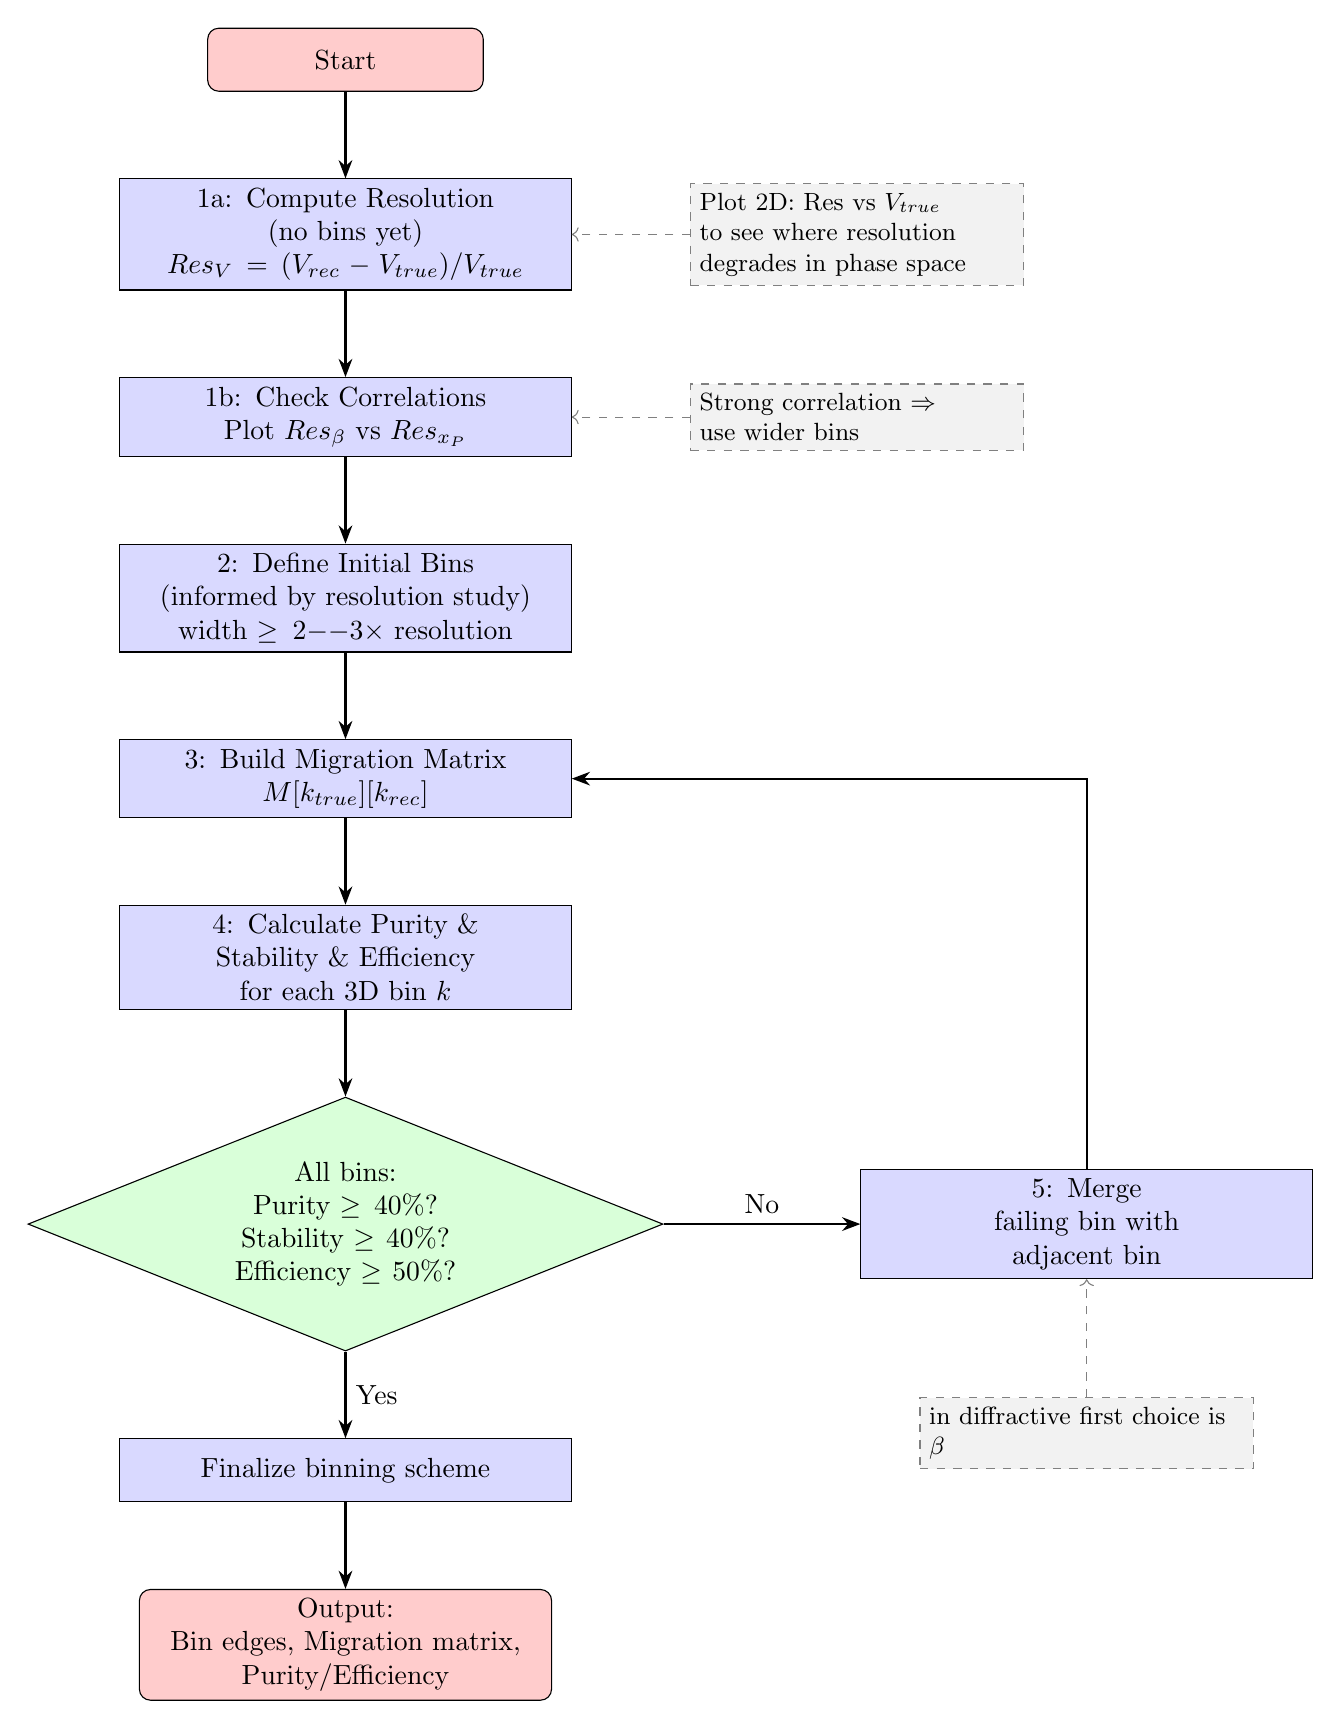
\begin{tikzpicture}[
      node distance=1.1cm,
      startstop/.style={rectangle, rounded corners, minimum width=3.5cm, minimum height=0.8cm, text centered, draw=black, fill=red!20},
      process/.style={rectangle, minimum width=5cm, minimum height=0.8cm, text centered, draw=black, fill=blue!15, text width=5.5cm},
      decision/.style={diamond, minimum width=3cm, minimum height=1cm, text centered, draw=black, fill=green!15, aspect=2.5, text width=2.5cm},
      arrow/.style={thick,->,>=Stealth},
      note/.style={rectangle, draw=gray, dashed, fill=gray!10, text width=4cm, font=\small}
  ]

  \node (start) [startstop] {Start};
  \node (res) [process, below=of start] {1a: Compute Resolution\\(no bins yet)\\$\text{Res}_V = (V_\text{rec} - V_\text{true})/V_\text{true}$};
  \node (note1) [note, right=1.5cm of res] {Plot 2D: Res vs $V_\text{true}$\\to see where resolution\\degrades in phase space};
  \node (corr) [process, below=of res] {1b: Check Correlations\\Plot $\text{Res}_\beta$ vs $\text{Res}_{x_\mathbb{P}}$};
  \node (note2) [note, right=1.5cm of corr] {Strong correlation $\Rightarrow$\\use wider bins};
  \node (initial) [process, below=of corr] {2: Define Initial Bins\\(informed by resolution study)\\width $\geq 2\text{--}3\times$ resolution};
  \node (migrate) [process, below=of initial] {3: Build Migration Matrix\\$M[k_\text{true}][k_\text{rec}]$};
  \node (purity) [process, below=of migrate] {4: Calculate Purity \& Stability \& Efficiency\\for each 3D bin $k$};
  \node (checkpur) [decision, below=of purity, text width=3.3cm, align=center] {All bins:\\Purity $\geq 40\%$?\\Stability $\geq 40\%$?\\Efficiency $\geq 50\%$?};
  \node (merge) [process, right=2.5cm of checkpur] {5: Merge\\failing bin with\\adjacent bin};
  \node (note3) [note, below=1.5cm of merge] {in diffractive first choice is $\beta$};
  \node (finalize) [process, below=of checkpur] {Finalize binning scheme};
  \node (output) [startstop, below=of finalize, text width=5cm, align=center] {Output:\\Bin edges, Migration matrix,\\Purity/Efficiency};

  \draw [arrow] (start) -- (res);
  \draw [arrow] (res) -- (corr);
  \draw [arrow] (corr) -- (initial);
  \draw [arrow] (initial) -- (migrate);
  \draw [arrow] (migrate) -- (purity);
  \draw [arrow] (purity) -- (checkpur);
  \draw [arrow] (checkpur) -- node[right] {Yes} (finalize);
  \draw [arrow] (checkpur) -- node[above] {No} (merge);
  \draw [arrow] (merge) |- (migrate);
  \draw [arrow] (finalize) -- (output);

  \draw [dashed, gray, ->] (note1) -- (res);
  \draw [dashed, gray, ->] (note2) -- (corr);
  \draw [dashed, gray, ->] (note3) -- (merge);

  \end{tikzpicture}
  }
\end{frame}

\begin{frame}[fragile]{Binning Scheme File (data/binning\_scheme.txt)}
  \small
  \verbatiminput{data/binning_scheme.txt}
  The global bin index for a 3D cell $(i, j, l)$ corresponding to $(Q^2_i
   , x_{\mathbb{P},j} , \beta_l)$ is:\\
  $k = l + j. N_\beta + i. N_\beta . N_{x_\mathbb{P}}$
\end{frame}

\begin{frame}{Purity / Stability / Efficiency (Q$^2$)}
  \begin{columns}
    \column{0.33\textwidth}
      \centering
      \includegraphics[width=\textwidth]{figs/binning/purity_vs_Q2.png}\\
      {\small Purity vs Q$^2$}
    \column{0.33\textwidth}
      \centering
      \includegraphics[width=\textwidth]{figs/binning/stability_vs_Q2.png}\\
      {\small Stability vs Q$^2$}
    \column{0.33\textwidth}
      \centering
      \includegraphics[width=\textwidth]{figs/binning/efficiency_vs_Q2.png}\\
      {\small Efficiency vs Q$^2$}
  \end{columns}
  \vspace{0.2cm}
  \small Bins with low efficiency are candidates for merging in the binning workflow.
\end{frame}

\begin{frame}{Purity / Efficiency (All 3D Bins)}
  \begin{columns}
    \column{0.5\textwidth}
      \centering
      \includegraphics[width=\textwidth]{figs/binning/purity.png}\\
      {\small Purity per 3D bin}
    \column{0.5\textwidth}
      \centering
      \includegraphics[width=\textwidth]{figs/binning/efficiency.png}\\
      {\small Efficiency per 3D bin}
  \end{columns}
  \vspace{0.2cm}
  \small Use these to identify bins failing the target criteria.
\end{frame}

\begin{frame}{Resolution (All Methods)}
  \centering
  \includegraphics[width=0.6\textwidth]{figs/binning/res_Q2.png}
  \vspace{0.2cm}
  \small $\mathrm{Res}_{Q^2} = (Q^2_\mathrm{rec} - Q^2_\mathrm{true})/Q^2_\mathrm{true}$
\end{frame}

\begin{frame}{Resolution (B0 / RP)}
  \begin{columns}
    \column{0.5\textwidth}
      \centering
      \includegraphics[width=\textwidth]{figs/binning/res_beta_B0.png}\\
      {\small $\beta$ resolution (B0)}
    \column{0.5\textwidth}
      \centering
      \includegraphics[width=\textwidth]{figs/binning/res_beta_RP.png}\\
      {\small $\beta$ resolution (RP)}
  \end{columns}
\end{frame}

\begin{frame}{Resolution (B0 / RP)}
  \begin{columns}
    \column{0.5\textwidth}
      \centering
      \includegraphics[width=\textwidth]{figs/binning/res_xpom_B0.png}\\
      {\small $x_{\mathrm{pom}}$ resolution (B0)}
    \column{0.5\textwidth}
      \centering
      \includegraphics[width=\textwidth]{figs/binning/res_xpom_RP.png}\\
      {\small $x_{\mathrm{pom}}$ resolution (RP)}
  \end{columns}
\end{frame}

\begin{frame}{Resolution Correlations}
  \begin{columns}
    \column{0.5\textwidth}
      \centering
      \includegraphics[width=\textwidth]{figs/binning/res_beta_vs_xpom_B0.png}\\
      {\small Res($\beta$) vs Res($x_{\mathrm{pom}}$) (B0)}
    \column{0.5\textwidth}
      \centering
      \includegraphics[width=\textwidth]{figs/binning/res_beta_vs_xpom_RP.png}\\
      {\small Res($\beta$) vs Res($x_{\mathrm{pom}}$) (RP)}
  \end{columns}
  \vspace{0.2cm}
  \small Correlations guide whether bins should be widened or merged.
\end{frame}

\begin{frame}{Binning Scheme Overlays}
  \begin{columns}
    \column{0.25\textwidth}
      \centering
      \includegraphics[width=\textwidth]{figs/binning/binning_Q2_vs_xpom.png}\\
      {\small Q$^2$ vs $x_{\mathrm{pom}}$}
    \column{0.25\textwidth}
      \centering
      \includegraphics[width=\textwidth]{figs/binning/binning_Q2_vs_beta.png}\\
      {\small Q$^2$ vs $\beta$}
  \end{columns}
  \vspace{0.2cm}
  \begin{columns}
    \column{0.25\textwidth}
      \centering
      \includegraphics[width=\textwidth]{figs/binning/binning_beta_vs_xpom.png}\\
      {\small $\beta$ vs $x_{\mathrm{pom}}$}
    \column{0.25\textwidth}
      \centering
      \includegraphics[width=\textwidth]{figs/binning/binning_Q2_vs_y.png}\\
      {\small Q$^2$ vs $y$}
  \end{columns}
\end{frame}

\end{document}
